%!TEX root = ../Thesis.tex
\chapter{Extra system graphics}
\begin{figure}[h]
    \centering
    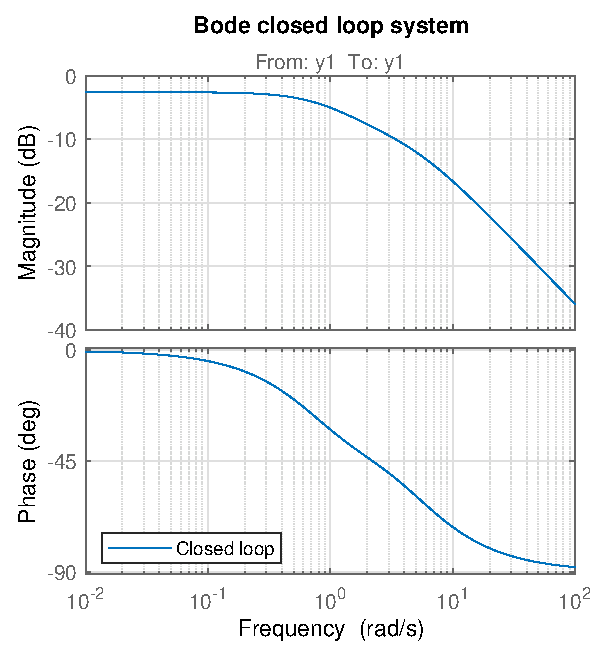
\includegraphics[width=0.9\textwidth]{figures/appendix/bode_closed_loop.eps}
    \caption{Closed loop frequency response (from $\omega_{ref}$ to $\omega_{out}$) of controlled system}
    \label{fig:systemcontrollerbode}
\end{figure}

\begin{figure}[h]
    \centering
    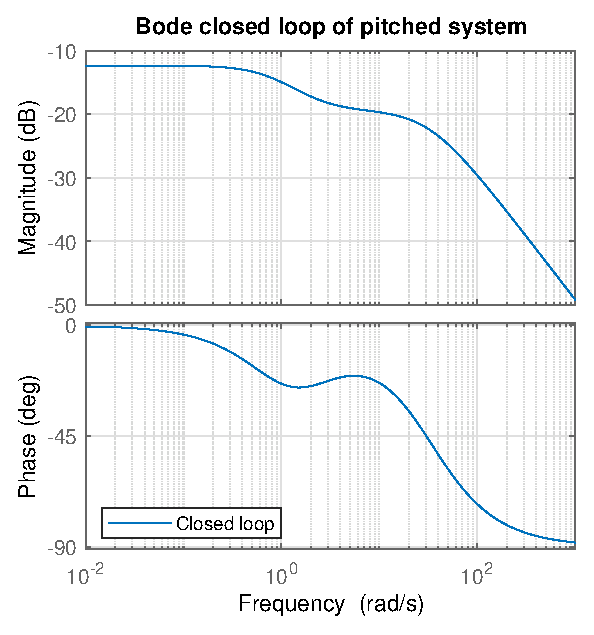
\includegraphics[width=0.9\textwidth]{figures/appendix/bode_closed_loop_pitch.eps}
    \caption{Closed loop frequency response (from $\omega_{ref}$ to $\omega_{out}$) of controlled system with pitched wings}
    \label{fig:systempitchcontrollerbode}
\end{figure}

\begin{sidewaysfigure}
    \centering
    \includegraphics[width=1\textwidth]{figures/system_modelling/top_level_block_diagram.PNG}
    \caption{Top level view of the Simulink model of the drone}
    \label{fig:toplevelmodel}
\end{sidewaysfigure}



\chapter{Video of flight test}
\href{https://youtu.be/Mw67W8S0a4E}{Link} to drone flight test: https://youtu.be/Mw67W8S0a4E\label{link:droneflight}

\chapter{Yaw drift test}
\begin{figure}[h]
    \centering
    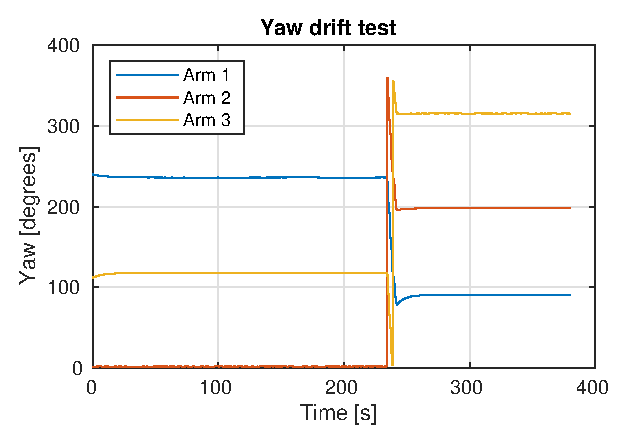
\includegraphics[width=0.9\textwidth]{figures/results/Yaw_drifttest.eps}
    \caption{Test of yaw drift. Measured for approximately 6 minutes. Manually did a rotation of about 170 degrees after 4 minutes}
    \label{fig:yawdrifttest}
\end{figure}